% No clue what this does
\documentclass{article}

% allow useage of graphics 
\usepackage[pdftex]{graphicx}
\usepackage{wrapfig}
%\usepackage[final]{graphicx}
%\usepackage[dvipdfmx]{graphicx} 
%\usepackage{bmpsize}

% Allow the usage of utf8 characters
\usepackage[utf8]{inputenc}

% Some maths package as it seemes
\usepackage{amsmath}
% For double line element like R, C or Z
\usepackage{amsfonts}
% For is defined as symbol (coloneqq)
\usepackage{mathtools}
% for Proof paragraphs
\usepackage{amsthm}

%subitem bulletpoints
\usepackage{outlines}

% bibtex style
\usepackage{apacite}

% a packages just used for the tabulator for the pascals triangle
\usepackage{array}

% package to alighn images
%\usepackage[export]{adjustbox}
\usepackage{float}
\usepackage{subcaption}

% use the tikz package, no clue why I need the positioning thing
\usepackage{tikz}
\usetikzlibrary{positioning}

% as it sais. Start the section counter from zero
% instead of starting it at one
\setcounter{section}{-1}

\theoremstyle{definition}
\newtheorem{theorem}{Theorem}[section]
\newtheorem{corollary}[theorem]{Corollary}
\newtheorem{lemma}[theorem]{Lemma}
\newtheorem{definition}[theorem]{Definition}
\newtheorem{proposition}[theorem]{Proposition}
\newtheorem{comment}[theorem]{Comment}
\newtheorem{remark}[theorem]{Remark}

% create a command to easyly add figure titles
\newcommand*{\figuretitle}[1]{%
    {\centering%   <--------  will only affect the title because of the grouping (by the
    \textbf{#1}%              braces before \centering and behind \medskip). If you remove
    \par\medskip}%            these braces the whole body of a {figure} env will be centered.
}

\title{Tropical Geometry of Deep Neural Networks}
\author{David Leatham}

% Start the document
\begin{document}


\maketitle

\newpage
  
\tableofcontents

\newpage


% Create a new 0th level heading named Intruduction
\section{Introduction}

\newpage

\section{Tropical Algebra}

%%%%%%%%%%%%%%%%%%%%%%%%%%%%%%%%%%
\tikzset{%
  every neuron/.style={
    circle,
    draw,
    minimum size=1cm
  },
  neuron missing/.style={
    draw=none, 
    scale=3,
    text height=0.333cm,
    execute at begin node=\color{black}$\vdots$
  },
}

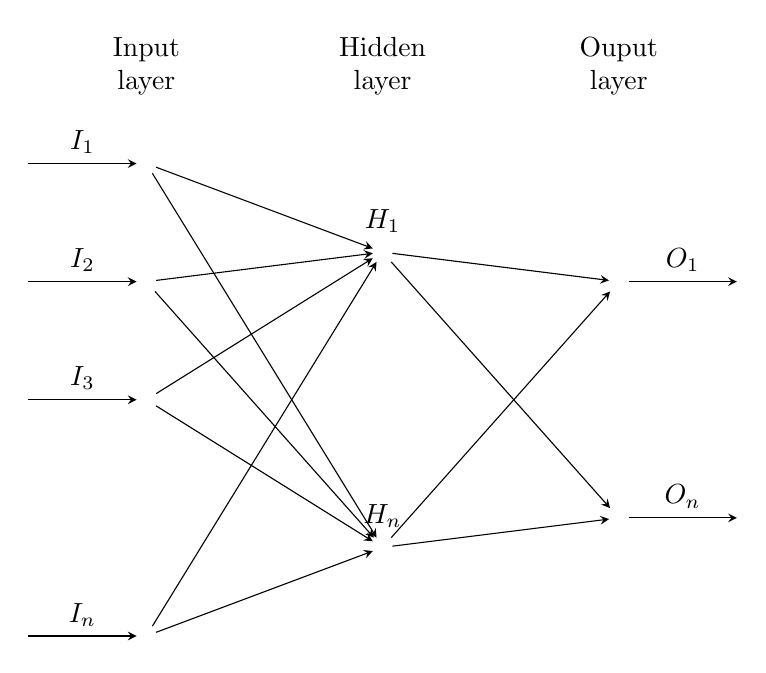
\begin{tikzpicture}[x=1.5cm, y=1.5cm, >=stealth]

\foreach \m/\l [count=\y] in {1,2,3,missing,4}
  \node [every neuron/.try, neuron \m/.try] (input-\m) at (0,2.5-\y) {};

\foreach \m [count=\y] in {1,missing,2}
  \node [every neuron/.try, neuron \m/.try ] (hidden-\m) at (2,2-\y*1.25) {};

\foreach \m [count=\y] in {1,missing,2}
  \node [every neuron/.try, neuron \m/.try ] (output-\m) at (4,1.5-\y) {};

\foreach \l [count=\i] in {1,2,3,n}
  \draw [<-] (input-\i) -- ++(-1,0)
    node [above, midway] {$I_\l$};

\foreach \l [count=\i] in {1,n}
  \node [above] at (hidden-\i.north) {$H_\l$};

\foreach \l [count=\i] in {1,n}
  \draw [->] (output-\i) -- ++(1,0)
    node [above, midway] {$O_\l$};

\foreach \i in {1,...,4}
  \foreach \j in {1,...,2}
    \draw [->] (input-\i) -- (hidden-\j);

\foreach \i in {1,...,2}
  \foreach \j in {1,...,2}
    \draw [->] (hidden-\i) -- (output-\j);

\foreach \l [count=\x from 0] in {Input, Hidden, Ouput}
  \node [align=center, above] at (\x*2,2) {\l \\ layer};

\end{tikzpicture}
%%%%%%%%%%%%%%%%%%%%%%%%%%%%%%%%%%%%%

Our basic object of study is the following object $( \mathbb{R} \cup \{- \infty \} , \oplus , \odot )$. As a set this is the real numbers $ \mathbb{R} $, together with an extra element $- \infty $ whitch represents minus infinity. In this (semiring) the tropical sum of real numbers is ther maximum and the tropical product of real numbers is their usual sum 
$$ x \oplus y := \max(x,\ y) \quad \& \quad x \odot y := x+y$$
--------------------------------------------------- \\
In Tropical Geometry often infinity instead of minus infinity and $\min$ in stead of $\max$ are used. This does not change any of the underlying theories of tropical algebra, as the the two semirings are tropically Isomorph. Meaning 
$$( \mathbb{R} \cup \{- \infty \} , \oplus := \max, \odot ) \to ( \mathbb{R} \cup \{ \infty \} , \oplus := \min , \odot ), x \mapsto \begin{cases} 
-x & x \in \mathbb{R}\\
\infty & x = - \infty
\end{cases}$$\\
is a tropical Isomorpism. \\
--------------------------------------------------- \\
First we will introduce the the tropical semiring and with it a usual semiring formally.
\begin{definition}
A semiring is a set $R$ equipped with two binary operations $+$ and $\cdot$, called addition and multiplication, such that (Wikipedia.en Semiring)
\begin{outline}
  \1 ($R$, $+$) is a cummutative monoid with identity element 0:
    \2 $(a + b) + c = a + (b + c)$
    \2 $0 + a = a + 0 = 0$
    \2 $a + b = b + a$
  \1 ($R$, $\cdot$) is a monoid with identity element $1$:
    \2 $(a \cdot b) \cdot c = a \cdot (b \cdot c)$
    \2 $ 1 \cdot a = a \cdot 1 = a $
  \1 Multiplication left and right distributes over addition
    \2 $ a \cdot (b + c) = (a \cdot b) + (a \cdot c)$
    \2 $ (a + b) \cdot c = (a \cdot c) + (b \cdot c)$
  \1 Multiplication by 0 annihilates
    \2 $ 0 \cdot a = a \cdot 0 = 0$
\end{outline}
\end{definition}

\begin{proposition}
$\mathbb{T} := ( \mathbb{R} \cup \{- \infty \} , \oplus , \odot )$ is a semiring called the tropical semiring. \cite[p.~10]{maclagan2015introduction}
\end{proposition}
\begin{proof}
~\
\begin{itemize}
\item[(1):]
The neutral element for the tropical sum is $- \infty$ since for $x \in \mathbb{R} \cup \{- \infty \}$ the following stands $ x \oplus \infty = \max(x,\ - \infty) = x$ and with $x \odot 0 = x + 0 = x$ for $x \in \mathbb{R}$, $0$ is the neutral elemet of tropical multiplication.
\item[(2):]
Both addition and multiplication are commutative. To prove this we take $x, y \in \mathbb{R} \cup \{- \infty \}$ and do a case distinct. Because $\mathbb{R}$ is a field w.l.o.g. we set $x= - \infty, y \in \mathbb{R}$
\begin{align*}
- \infty \oplus y = \max (- \infty ,\ y) &=   y = \max ( y,\ - \infty ) = y \oplus \infty \\
\infty \odot y = \infty +y &= \infty = y+ \infty = y \odot \infty
\end{align*}
\item[(3):]
Tropical multiplication distributes over addition. Take $x, y, z \in \mathbb{R}$ then
\begin{align*}
x \odot (y \oplus z) = x + \max (y,\ z) &=   \max (x + y,\ x + z) = (x \odot y) \oplus (x \odot z) \\
(y \oplus z) \odot x = \max (y,\ z) + x &=   \max (y + x,\ z + x) = (y \odot x) \oplus (z \odot x)
\end{align*}
\item[(4):]
Multiplication by $- \infty$ annihilates $- \infty \odot x = - \infty \: \forall x \in  \mathbb{R} \cup \{- \infty \}$.
\end{itemize}
\end{proof}

An essential feature of tropical arithmetics is that there is no subtraction. Take $a, b \in \mathbb{R} \cup \{- \infty \}$ with $a < b$ then the equation $a \oplus x=b$ has no solution x at all. \cite[p.~11]{maclagan2015introduction} \\ \\

To get more familiar with the tropical arithmetics we will have a look at an arithemtical example, before we jump into tropical polynomials.
\begin{remark}
The tropical Pascal’s triangle, whose rows are the coefficients appearing in a binomial expansion, is very simple to remember. All its coefficients are Zero.
For example, the fourth row in the triangle is represented be the following equation 
\begin{align*}
(a \oplus b)^{3} &= 3 \max (a , b) \\
&= \max (3a, 3b) = (a^{3} + b^{3}) \\
&= \max (0 \odot a^{3} , 0 \odot a^{2} \odot b , 0 \odot a \odot b^{2} , 0 \odot b^{3}) \ with \ a, b \in \mathbb{T}
\end{align*}
You may say the Pascal's coefficients are four zeroes. The same applies to all cases
\begin{align*}
(a \oplus b)^{n} &= a^{n} \oplus b^{n} \\
&= 0a^{n} \oplus 0a^{n-1}b \oplus \dots \oplus 0ab^{n-1} \oplus b^{n}.
\end{align*}
And Pascal's triangle has the following form. \\ \\
\begin{tabular}{>{$n=}l<{$\hspace{12pt}}*{13}{c}}
0 &&&&&&&$0$&&&&&&\\
1 &&&&&&$0$&&$0$&&&&&\\
2 &&&&&$0$&&$0$&&$0$&&&&\\
3 &&&&$0$&&$0$&&$0$&&$0$&&&\\
4 &&&$0$&&$0$&&$0$&&$0$&&$0$&&\\
5 &&$0$&&$0$&&$0$&&$0$&&$0$&&$0$&\\
6 &$0$&&$0$&&$0$&&$0$&&$0$&&$0$&&$0$.
\end{tabular}
\end{remark}

The goal of this first section and the following is to get to understand tropical rational functions and < maps, as the underlying objects are key to later relations between neural networks and Tropical Geometry. Linking these two field is  core to this thesis. \
First, so that we can introduce multidimensional tropical polynomials properly a notion of monomials is needed.

\begin{definition}
\cite[p.~2]{zhang2018tropical}
A tropical monomial in d variables $x_1 , \dots , x_d$ is an expression or function $ \mathbb{T}^{d} \to \mathbb{T} $ of the from 
$$ c \odot x_1^{a_1} \odot x_2^{a_2} \odot \dots \odot x_{d-1}^{a_{d-1}} \odot x_d^{a_d}$$
where $c \in \mathbb{R} \cup \{- \infty \}$ and $a_1, \dots , a_d \in \mathbb{N}$. As a convenient shorthand, we will also write a tropical monomial in multiindex notation as $cx_{\alpha}$ where $\alpha = (a_1 , \dots , a_d) \in \mathbb{N}_d$ and $x = (x_1 , \dots , x_d)$. Note that $x^{\alpha} = 0 \odot x^{\alpha}$.
\end{definition}

\begin{definition}\label{tropPolyn}
\cite[p.~2]{zhang2018tropical}
Following notations above, a tropical polynomial $f(x)=f(x_1, \dots , x_d), f: \mathbb{T}^{d} \to \mathbb{T}$ is a finite tropical sum of tropical monomials 
$$ f(x)=c_1x^{\alpha_1} \oplus \dots \oplus c_rx^{\alpha_r}$$
where $\alpha_i = (\alpha_{i1}, \dots , \alpha_{id}) \in \mathbb{N}^{d}$ and $c_i \in \mathbb{R} \cup \{- \infty \}$, $i = 1, \dots , r$. We will assume that a monomial of a given multiindex appears at most once in the sum, i.e. $\alpha_i \neq \alpha_j$ for any $i \neq j$.
\end{definition}

\begin{remark}
We are going to examine tropical polynomials in one variable. Monomials in one variable are of the form $ c \odot x^{a}, \mathbb{T} \to \mathbb{T}$ where $c \in \mathbb{T}$ and $ a \in \mathbb{N} $. Meaning a tropical polynomial in one variable is of the form $f(x)=c_1x^{\alpha_1} \oplus \dots \oplus c_rx^{\alpha_r} \ with \ c_i \in \mathbb{T}, a_i \in \mathbb{N} \ for \ i=1, \dots , r$. \\
For a quadratic tropical polynomial $f(x) = a \oplus bx \oplus cx^{2} with a,b,c \in \mathbb{T}$ linearity breaks at two points $b-c$ and $a-b$ if $b-c > a$, otherwise it only breaks at one point $(a-c):2$. Visualising two quadratic tropical functions gives a good intuition of the piecewise-linearity. \\
The black colored parts of the followig figures one and two indicate the graph of the tropical polynomial.

\begin{figure}[h]

\begin{subfigure}{0.5\textwidth}
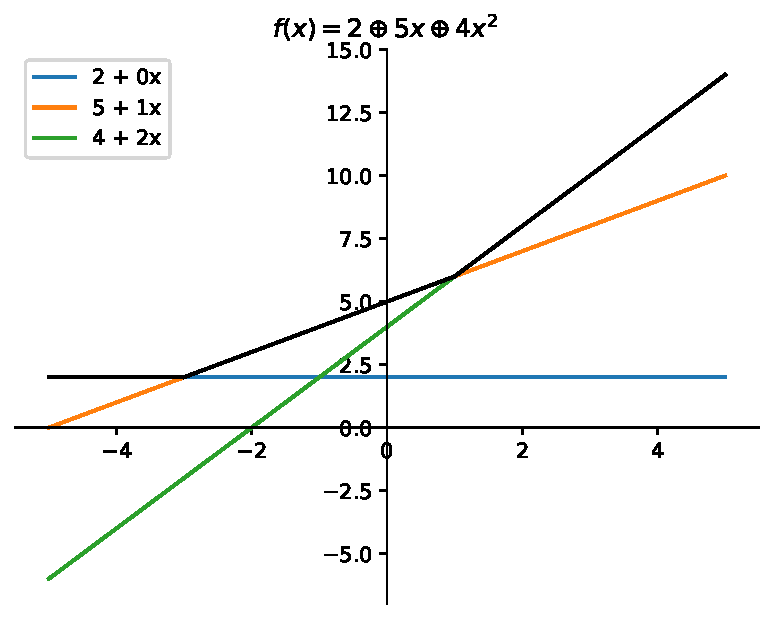
\includegraphics[scale=0.5]{graphics/first_trop_pol.pdf}
\caption{Take $f(x) = 2 \oplus 5x \oplus 4x^{2}$ a quadratic polynomial. The graph equals $max(2, 5+x, 4+2x)$. Until $5-2$, $2$ dominates, from there $5+x$ dominates to the point $4+2x$.}
\label{fig:fs_mi}
\end{subfigure}
\begin{subfigure}{0.5\textwidth}
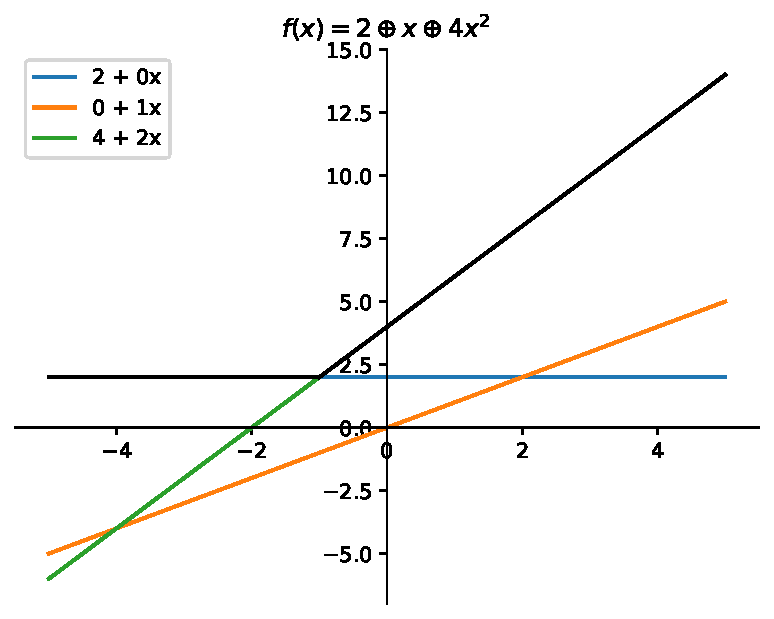
\includegraphics[scale=0.5]{graphics/second_trop_pol.pdf}
\caption{Take $f(x)=2 \oplus x \oplus 4x^{x}$, we have changed the scalar in the second part, then this second part plays no part in the tropical polynomial.}
\label{fig:fs_mi}
\end{subfigure}

\caption{Quadratic tropical polynomials.}
\label{fig:image2}
\end{figure}

We can see the degree of a tropical polynomial, defined the same as a degree of a usual polynomial, gives an upper bound for the number of non linear edges of the tropical polynomial, but not the exact value. With higher degree polynomials more non linear edges are possible:


\begin{figure}[H]
\centering
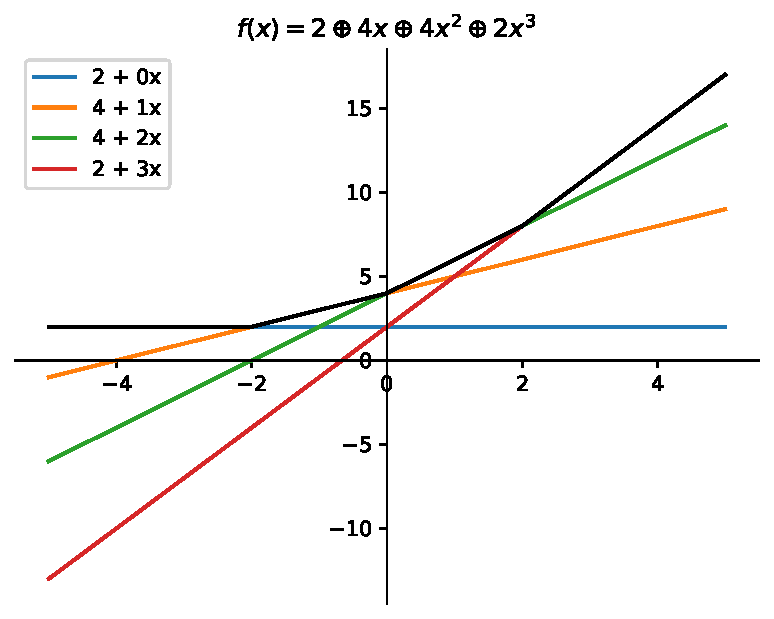
\includegraphics[scale=0.75]{graphics/third_trop_pol.pdf}
\caption{Take $f(x)=2 \oplus x \oplus 4x^{x} \oplus 4x^{2} \oplus 3x^{3}$. For a degree three tropical polynomial in one variable this polynomial has reached the maximum number of non linear edges.}
\label{fig:fs_mi}
\end{figure}


\end{remark}

In multiple variables we can characterise tropical polynomials as functions from $\mathbb{R}^{n} \to \mathbb{R}$ that satisfy the following three properties.

\begin{lemma}\label{lemma:trop_properties}
Let f be a tropical polynomial
$$ f(x) = c_1^{\alpha_1} \oplus \dots \oplus c_r x^{\alpha_r}$$ as in \ref{tropPolyn}. Then f has three important properties:
\begin{itemize}
\item[(1)]
$f$ is continuous.
\item[(2)]
$f$ is piecewise-linear, where the number of pieces is finite.
\item[(3)]
$f$ is convex, i.e. $p(\frac{x + y}{2}) \leq \frac{1}{2}(p(x)+p(y)) \forall x,y \in \mathbb{R}$
\end{itemize}
\end{lemma}

\begin{proof}
(1) The minimum of continuous functions is still continuous. \\
(2) Every monomial $c_ix^{\alpha_i} = c_i + xy\alpha_{i1} + \dots + x_r \alpha_{ir}$ is per definition linear. Because of (1), linearity can only be broken where $c_i x^{\alpha_i} = c_j x^{\alpha_j}$ for $i \leq j$ and $i,j = 1, \dots ,r$. \\
A piece is a single piece of $c_ix^{\alpha_i}$ where linearity is not broken. If we introduce $c_ix^{\alpha_i}$ one after another, then in the $i$-th step not more than $i^2$ new pieces can be created, so there can only be $\displaystyle \sum_{i=1}^{r} i^2$ or less pieces. \\
(3) On one piece f is convex. Moving from one piece to another the slope can only increase, with means f is still convex.
\end{proof}

\begin{proposition}
Every function $\mathbb{R}^{n} \to \mathbb{R}$ which satisfies the three properties (1), (2) and (3) has a representation as the minimum of a finite set of linear functions. Thus, the tropical polynomial in n variables $x_{1}, \dots x_{n}$ represent the class of piecewise-linear convex functions on $\mathbb{R}^{n}$ with integer coefficients.
\end{proposition}

\begin{proof}
This follows directly from lemma \ref{lemma:trop_properties}.
\end{proof}

Now we are ready to introduce tropical rational functions. These are important to understand the core section, section \ref{sec:trop_netw}, in particular the actual connection build between neural networks and tropical geometry in this thesis, as are the semifields $\mathbb{T}[X_{1} , \dots , X_{d}]$ and $\mathbb{T}(X_{1} , \dots , X_{d})$.

\begin{definition} \cite[p.~3]{zhang2018tropical}
Following notations above, a tropical rational function is a standard difference, or, equivalently,
a tropical quotient of two tropical polynomials $f(x)$ and
$g(x)$:
$$ (f-g)(x) = f(x) - g(x) = f(x) \oslash g(x) = (f \oslash g)(x)$$
%We will denote a tropical rational function by $f \oslash g$, where $f$ and $g$ are understood to be tropical polynomial functions.
\end{definition}



\begin{proposition}
$\mathbb{T}[X_1, \dots , X_d] := \{ f: \mathbb{T}^{d} \to \mathbb{T} ; f \ is \ tropical \ polynomial \}$ and \ $ \mathbb{T}(X_1, \dots , X_d) := \{ f: \mathbb{T}^{d} \to \mathbb{T} ; f \ is \ tropical \ rational \ function \}$ are both semifields. \cite[p.~3]{zhang2018tropical}
\end{proposition}
\begin{proof}
Let $g,f,h \in \mathbb{T}(X_1, \dots ,X_d)$ with 
\begin{align*}
f(x) &= f_1(x) \oslash f_2(x) = (\oplus_{i=0}^r c_{1i} x^{\alpha_{1i}}) \oslash (\oplus_{i=0}^r c_{2i} x^{\alpha_{2i}}) \\
g(x) &= g_1(x) \oslash g_2(x) = (\oplus_{i=0}^r d_{1i} x^{\beta_{1i}}) \oslash (\oplus_{i=0}^r d_{2i} x^{\beta_{2i}}) \\
h(x) &= h_1(x) \oslash h_2(x) = (\oplus_{i=0}^r e_{1i} x^{\gamma_{1i}}) \oslash (\oplus_{i=0}^r e_{2i} x^{\gamma_{2i}}) \\
\end{align*}
We begin the proof by showing, that for two tropical polynomials $a(x)= \oplus_{i=0}^r z_{i} x^{\zeta_{i}}), b(x)= \oplus_{i=0}^r o_{i} x^{\omega_{i}}) \in \mathbb{T}[X_1, \dots , X_r]$ the normal sum is a tropical polynomial $(a + b)(x) \in \mathbb{T}[X_1, \dots , X_r]$.
\begin{align*} 
(a + b)(x) &= a(x) + b(x) \\
&=  (\oplus_{i=0}^r z_{i} x^{\zeta_{i}}) + (\oplus_{i=0}^r o_{i} x^{\omega_{i}}) \\
&= \oplus_{i, j = 0, \dots , r} (z_{i} + \zeta_{i} * x + o_{j} + \omega_{i} * x) \\
&= \oplus_{i, j = 0, \dots , r} ((z_{i} + o_{j}) + x^{\zeta_{i} + \omega_{i}}) \in \mathbb{T}[X_1, \dots X_r]
\end{align*}
Other than with the proof of the Tropical semiring we will show that topical tropical addition and tropical multiplication of tropical polynomials as tropical rational functions stay tropical polynomials respectively tropical rational functions. All other axioms stay pointwise the same.
\begin{itemize}
\item[(1):]
The Tropical sum of a Tropical rational functions is a tropical tropical rations function
\begin{align*}
(f \oplus g)(x) &= f(x) \oplus g(x) \\
&=(f_1(x) \oslash f_2(x)) \oplus (g_1(x) \oslash g_2(x)) \\
&= \min\{f_1(x) - f_2(x), g_1(x) - g_2(x) \} \\
&= \min\{f_1(x) + g_2(x), g_1(x) + f_2(x) \} - f_2(x) - g_2(x) \\
&= (f_1(x) + g_2(x) \oplus g_1(x) + f_2(x)) \oslash (f_2(x) + g_2(x)) \in \mathbb{T}(X_1, \dots , X_r).
\end{align*}
Since Addition as tropical addition of tropical polynomials is a tropical polynomial.
\item[(2):]
The Tropical product of a Tropical rational functions is a tropical tropical rational function
\begin{align*}
(f \odot g)(x) &= f(x) \odot g(x) \\
&=  (f_1(x) \oslash f_2(x)) \odot (g_1(x) \oslash g_2(x)) \\
&= f_1(x) - f_2(x) + g_1(x) - g_2(x) \\
&= (f_1(x) + g_1(x)) - (f_2(x) + g_2(x)) \in \mathbb{T}(X_1, \dots , X_r)
\end{align*}
\item[(3):]
The neutral element for the tropical sum is $- \infty = - \infty \oslash x = x \oslash - \infty \ x \in \mathbb{T}$ since for $f(x) \in \mathbb{T}(X_1, \dots , X_r)$ as above, the following stands $ f(x) \oplus \infty = \max(f(x),\ - \infty) = f(x)$ and with $f(x) \odot 0 = f(x) + 0 = f(x) \forall f(x) \in \mathbb{T}$ $0$ is the neutral element of tropical multiplication.
\end{itemize}
\end{proof}

\begin{comment}
We regard a tropical polynomial $f=f \oslash 0$ as a special case of a tropical rational function and thus $\mathbb{T}[X_1, \dots , X_r] \subseteq \mathbb{T}(X_1, \dots , X_r)$ \cite[p.~3]{zhang2018tropical}.
\end{comment}

\begin{comment}
~\
\begin{itemize}
\item[$\bullet$]
A d-variate tropical polynomial $f(x)$ defines a function $f: \mathbb{T}^{d} \to \mathbb{T}$ that is a convex function in the usual sense as taking $\max$ and $\sum$ of convex functions preserve convexity \cite{boyd2004convex}.
\item[$\bullet$]
As such, a tropical rational function $f \oslash g : \mathbb{T}^{d} \to \mathbb{T}$ is a DC function or differenceconvex function \cite{hartman1959functions}.
\end{itemize}
\end{comment}

\begin{remark}
The only thing missing to this section are some examples for tropical rational functions and tropical rational maps. \\
!!! Expand by adding some examples !!!
\end{remark}

\begin{definition}
$R : \mathbb{R}^{d} \to \mathbb{R}^{p}, x = (x_1, \dots , x_d)\mapsto (f_1(x), \dots , f_p(x))$, is called a tropical polynomial map if each $f_i : \mathbb{R}^{d} \to \mathbb{R}$ is a tropical polynomial, $i = 1, \dots , p$, and a tropical rational map if $f_1, \dots , f_p$ are tropical rational functions. We will denote the set of tropical polynomial maps by $Pol(d, p)$ and the set of tropical rational maps by $Rat(d, p)$. So $Pol(d, 1) = \mathbb{T}[X_1, \dots , x_d]$ and $Rat(d, 1) = \mathbb{T}(x_1, \dots , x_d)$ \cite[p.~3]{zhang2018tropical}.
\end{definition}

\newpage

\section{Tropical hypersurfaces}

\begin{definition}
The tropical hypersurface of a tropical polynomial $f(x) = c_1 x^{\alpha_1} \oplus \dots \oplus c_r x^{\alpha_r}$ is 
$$\Gamma(f) := \{ x \in \mathbb{R}^{d} : c_i x^{\alpha_i} = c_j x^{\alpha_j} = f(x) for some \alpha_i \neq \alpha_j \}$$
i.e., the set of points x at which the value of f at x is attained by two or more monomials in f \cite[p.~3]{zhang2018tropical}.
\end{definition}

\begin{comment}
A tropical polynomial $f$ determines a dual subdivision of
$\delta (f)$, constructed as follows. First, lift each $\alpha_i$ from $\mathbb{R}^d$ into $\mathbb{R}^{d+1}$ by appending $c_i$ as the last coordinate. Denote the convex hull of the lifted $\alpha_1, \dots , \alpha_r$ as
$$\mathcal{P}(f):= Conv{(\alpha_i, c_i) \in \mathbb{R}^{d} \times \mathbb{R} : i = 1, \dots , r}. (1)$$
Next let $UF(\mathcal(P)(f))$ denote the collection of upper faces in $\mathcal{P}(f)$ and $\pi : \mathbb{R}^{d} \times \mathbb{R} \to \mathbb{R}^{d}$ be the projection that drops
the last coordinate. The dual subdivision determined by $f$
is then
$$\delta(f) := {\pi(p) \subset \mathbb{R}^{d} : p \in UF( \mathcal{P}(f))}.$$.
$\delta (f)$ forms a polyhedral complex with support $\delta (f)$. By \cite{maclagan2015introduction}, the tropical hypersurface $\mathcal{T}(f)$ is the $(d - 1)$-skeleton of the polyhedral complex dual to $ \delta(f)$. This means that each vertex in $ \delta(f)$ corresponds to one "cell" in $R^{d}$ where the function f is linear. Thus, the number of vertices in $\mathcal{P}(f)$ provides an upper bound on the number of linear regions of $f$.
\end{comment}

\begin{definition}
The Newton polygon of a tropical polynomial $f(x) = c_1 x^{\alpha_1} \oplus \dots \oplus c_r x^{\alpha_r}$  is the convex hull of $\alpha_1 , \dots , \alpha_r \in \mathbb{N}^{d}$, regarded as points in $\mathbb{R}^{d}$,
$$ \Delta(f) := Conv{\alpha_i \in \mathbb{R}^{d} : c_i \neq -\infty , i = 1, \dots ,r } $$ \cite[p.~3]{zhang2018tropical}.
\end{definition}

\begin{definition}
A linear region of $F \in Rat(d, m)$ is a maximal connected subset of the domain on which $F$ is linear. The number of linear regions of $F$ is denoted $\mathcal{N}(f)$ \cite[p.~4]{zhang2018tropical}.
\end{definition}

\subsection{Transformations of tropical polynomial}

\begin{proposition}
Let $f$ be a tropical polynomial and let $a \in \mathbb{N}$. Then
$$ \mathcal{P}(f^{a}) = a \mathcal{P}(f) $$.
$a \mathcal{P}(f) = \{ax : x \in \mathcal{P}(f) \} \subset \mathbb{R}^{d + 1}$ is a scaled version of $\mathcal{P}(f)$ with the same shape but different volume \cite[p.~4]{zhang2018tropical}.
\end{proposition}
\begin{proof}
\end{proof}

\begin{definition}
The Minkowski sum of two sets $P_1$ and $P_2$ in $\mathbb{R}^{d}$ is the set
$$ P_1 + P_2 := \{x_1 + x_2 \in \mathbb{R}^{d} : x_1 \in P_1 ,x_2 \in P_2 \} $$;
and for $\lambda_1 , \lambda_2 \geq 0$, their weighted Minkowski sum is
$$ \lambda_1 P_1 + \lambda_2 P_2 := \{ \lambda_1 x_1 + \lambda_2 x_2 \in \mathbb{R}^{d} : x_1 \in P_1 , x_2 \in P_2 \} $$ \cite[p.~4]{zhang2018tropical}.
\end{definition}

\begin{proposition} \cite[p.~4]{zhang2018tropical}
Let $f, g \in Pol(d, 1) = \mathbb{T}[x_1, \dots , x_d]$ be tropical polynomials. Then
\begin{align*}
\mathcal{P}(f \odot g) &= \mathcal{P}(f) + \mathcal{P}(g),
\mathcal{P}(f \oplus g) &= Conv(\mathcal{V}(\mathcal{P}(f)) \cup \mathcal{V}( \mathcal{P}(g))).
\end{align*}
\end{proposition}

\begin{theorem}
(Gritzmann-Sturmfels). Let $P_1, \dots , P_k$ be polytopes in $\mathbb{R}^{d}$ and let m denote the total number of nonparallel edges of $P_1, \dots , P_k$. Then the number of vertices of $P_1 + \dots + P_k$ does not exceed
$$\sum_{j=0}^{d-1} \binom{m-1}{j}.$$
The upper bound is attained if all $P_i$'s are zonotopes and all their generating line segments are in general positions. \cite{gritzmann1993minkowski}
\end{theorem}

\begin{corollary}
Let $\mathcal{P} \in \mathbb{R}^{d+1}$ be a zonotope generated by m line segments $P_1 , \dots , P_m$. Let $\pi : \mathbb{R}^{d} \times \mathbb{R} \to \mathbb{R}^{d}$ be the projection. Suppose $P$ satisfies:
\begin{itemize}
\item[(i)]
the generating line segments are in general positions;
\item[(ii)]
the set of projected vertices $\{ \pi(v) : v \in \mathcal{V}(\mathcal{P}) \} \subseteq \mathbb{R}^{d}$ are in generalposition.
\end{itemize}
Then $P$ has
$$ \sum_{j=0}^{d} \binom{m}{j} $$
vertices on its upper faces. If either (i) or (ii) is violated, then this becomes an upper bound. \cite[p.~4]{zhang2018tropical}
\end{corollary}

\newpage

\section{Neural networks}

Neural networks viewed as a topic, make for a very compelling field of interest in their own right. Historically the term "Neural Network" was introduced in attempts to describe the functionality of biological processes, in particular the nervous system and the brain, in a mathematical sense \cite{mcculloch1943logical, widrow1960adaptive, rumelhart1986learning}. Simplified the nervous system is a net of neurons, each having a soma and an axon. At any instant a neuron has some threshold, which excitation must exceed to initiate an impulse. This, except for the fact and the time of its occurrence, is determined by the neuron, not by the excitation. From the point of excitation the impulse is propagated to all parts of the neuron \cite{mcculloch1943logical}. Through synapses the axons are connected to further soma through with the impulse is passed on to further neurons. Impulses passing through the nervous system partly consist of electrical impulses and chemical reactions \cite{palay1956synapses}. A collection of partially connected neurons, capable of carrying impulses, is called a biological neural network.


\begin{figure}[H]
\centering
\figuretitle{Depiction of a neuron}
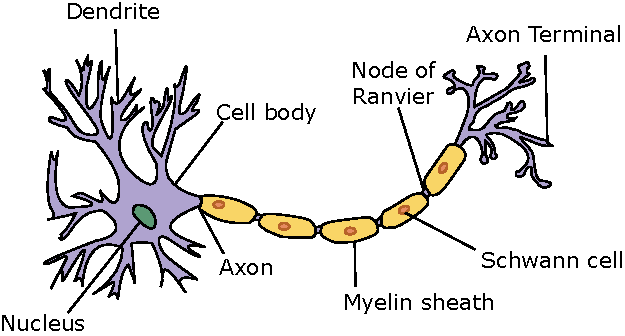
\includegraphics[scale=0.75]{graphics/neuron.pdf}
\caption{A representation of a neuron. The axon terminal attach to dendrite. This way impulses pass from neuron to neuron.}
\label{fig:neuron}
\end{figure}

In reference to a biological neural network, an abstract neuronal network, in the following simply referenced as neuronal networks, are defined. As a biological neuron and especially a biological neural network is far more complex than this introduction may make it seem, biological realism would impose entirely unnecessary constraint. Boiling a biological neuronal network down to its quintessential features results in a weighted directed graph, where edges and vertices are weighted. Typically a weighted graph only has its edges weighted. To fit our model better we introduce them also with weighted vertices.

\begin{definition}
A graph is a pair $G = (V, E)$, where $V$ is a set whose elements are called vertices, and $E \subset \{ {x, y}|(x,y) \in v^{2} \}$ is a set of two-sets of vertices, whose elements are called edges.
\end{definition}

\begin{definition}
A directed graph is a pair $G = (V, E)$, where $V$ is a set whose elements are called vertices, and $E \subset \{ (x, y)|(x,y) \in v^{2} \}$ is a set of edges which are ordered pairs of distinct vertices.
\end{definition}

\begin{definition}
A weighted graph $G = (V, E)$ in our case is attributed by two functions $\psi : V \to \mathbb{K}$ and $\omega : E \to \mathbb{K}$ that assign a weight $\psi(v)$ and $\omega(e)$ to each edge $e \in E$ and weight $v \in V$, with $\mathbb{K}$ being a field.
\end{definition}

\begin{definition}
Let $G = (V, E)$ be a Graph. We set $n(G) = |V|$ to be the cardinality of vertices and $m(G) = |E|$ the cardinality of edges.
\end{definition}

Graphs can represent a multitude of relations between objects. Like road maps of roads connecting cities. Or describe objects them selves like molecules.

\begin{remark}
For instance the following weighted directed Graph could depict a road map with cities as nodes connected by roads that are weighted with the distance between cites and we want to find the minimal distance from any city to city A. \

\begin{figure}[H]
\centering
\figuretitle{Min distance weighted graph}
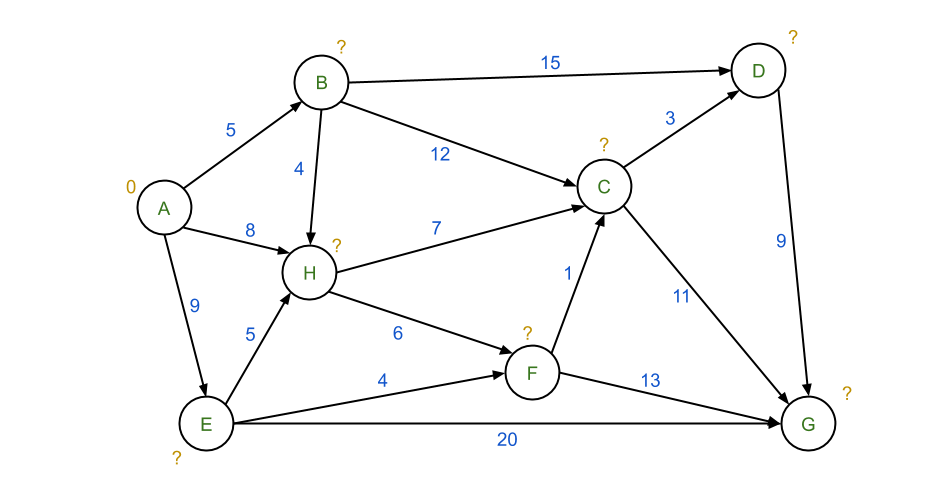
\includegraphics[scale=0.5]{graphics/weighted_directed_graph_2.png}
\caption{Min distance weighted graph.}
\label{fig:neuron}
\end{figure}

In a graph where we have a way to reach each node from the starting point, as our graph has this property, Dijkstra's algorithm gives us, for small graphs, an easy algorithm to compute the shortest path from node A to any other node by hand. At any point in the algorithm simply consider all reachable nodes from nodes that have their shortest path already computed by adding up the shortest paths length to the previous node and the path length of the path between the nodes. This way every reachable node by nodes with there shortest path already computed get at least one or multiple lengths of paths assigned to them. Pick the shortest path under all of these and repeat until all vertices have a path assigned. If there are multiple shortest paths, pick one of them. \\
We will proof that this gives us a correct result through induction.
\begin{proof} 
For each node $v$, $dist(v)$ is the shortest distance from source to $v$ when traveling via visited nodes only, or infinity if no such path exists. (Note: we do not assume $dist(v)$ is the actual shortest distance for unvisited nodes.) \\
The base case is when there is just one visited node, namely the initial node source, in which case the hypothesis is trivial. \\
Otherwise, assume the hypothesis for $n-1$ visited nodes. In which case, we choose an edge $vu$ where $u$ has the least $dist(u)$ of any unvisited nodes and the edge $vu$ is such that $dist(u) = dist(v) + length(v,u)$. $dist(u)$ is considered to be the shortest distance from source to $u$ because if there were a shorter path, and if $w$ was the first unvisited node on that path then by the original hypothesis $dist(w) > dist(u)$ which creates a contradiction. Similarly if there were a shorter path to u without using unvisited nodes, and if the last but one node on that path were $w$, then we would have had $dist(u) = dist(w) + length(w,u)$, also a contradiction. \\
After processing $u$ it will still be true that for each unvisited node $w$, $dist(w)$ will be the shortest distance from source to $w$ using visited nodes only, because if there were a shorter path that doesn't go by $u$ we would have found it previously, and if there were a shorter path using u we would have updated it when processing $u$. \\
After all nodes are visited, the shortest path from source to any node $v$ consists only of visited nodes, therefore $dist(v)$ is the shortest distance.
\end{proof}

Now that we understand Dijkstra's algorithm, to complete the remark, we will compute the shortest distance to vertex $C$, by terminating Dijkstra's algorithm as soon as we have computed the shortest path to $C$. \\
From $A$ the shortest distance to adjacent vertices is the distance to vertex $B$ with length $5$. We set the shortest distance to $B$ to $5$ and repeat. This time we have to also consider the the distances to adjacent vertices to $B$ with the added shortest distance to $B$. So in this iteration paths of length $20$ to $D$, $17$ to $C$ and $9$ to $H$ with is closely beaten by $8$ to $H$ from $A$ are to be considered. We mark $8$ to be the shortest distance to $H$. We describe one more step in detail and let the reader confirm if the calculated value for $C$ is correct. We have now computed the minimal distance to nodes $A$, $B$ and $H$. Reachable nodes at this point are $D$, $C$, $F$ and $E$ with path lengths of $20, 17, 15, 14$ and $9$. $9$ is the shortest, the shortest way to node $E$ is of length $9$. Next is node $F$ and then $C$ with it's length being $14$.

\end{remark}

------------------------------------ \\
One more nice thing to do would be to elaborate and introduce a neural network, that does not have a specific input or out. For example no output. Right now I have no inspiration for this specific topic, so I will go on. \\
------------------------------------

Graph theory is a big field, but we are interested in modelling neural networks. In particular in those neural networks that have specific input layers and output layers. Our goal at this point is to get an insight of how to construct a neural network and define weights, so that our output stands in a predefined relation to our input.
In particular one of the most important neural networks is the L-layer feedforward neural network. \
We will define and motivate L-layer feedforward neural networks using graphs at first and then abstract again to only their necessary features.

\begin{definition}
An $L$-layer feedforward neural network in graph form $(G, \sigma)$ is a weighted graph $G$ with an activation function $\sigma$. The graph consists of $L$ sets $V^{(j)}$, $j = 1, \dots , L$ of vertices with $L-1$ corresponding sets of edges $E^{(i)} \subset \{(x,y)|x \in V^{(i)}; y \in V^{(i+1)}\}$, $i = 1, \dots , L-1$ which connect two consecutive layers.  The Graph of a $0$-layer feedforward neural network is an empty graph and of a $1$-layer feedforward neural network is a set of vertices without connecting edges.
\end{definition}

\begin{remark}
The first layer of an $L$-layer feedforward neural network is called the input layer and the last ($L$-th) layer is called the output layer. All layers in between collectively are called hidden layers.
\end{remark}

\begin{remark}
A fully connected feedforward neural network $(G, \sigma)$ with $G = (V, E)$ is one where $E$ is the largest out of every possible set of $E$. This will give the unique solution, where $V^{(j)}$ and $V^{(j+1)}$ for each $j = 1, \dots , L-1$ will be fully connected.
\end{remark}

We are at an interesting point of this chapter. Inspired by biological neural networks, which are the core building blocks of animal brains, we have abstracted some of the essential features, given an introduction to graphs and used these as a mathematical buildingblock for neural networks.
With the introduction of feed forward neural networks we have cast an sensible form of neural network with is able to store and also learn complex relations between input data and output data through forward and backward propagation. \\
Forward propagation describes the process by which from an input vector the output vector is calculated. First we need to introduce the bias and weight vector $W^{(j)}$.

\begin{remark}\label{standardGraphLabeling}
Let $(G, \sigma)$ be a $L$-layer feedforward neural network where we fixate the elements from the sets $V^{(j)}$, by naming them $b_{j1}$ to $b_{j|V^{(j)}|}$, so that we can establish a correlating vector $b^{(j)} = (b_{j1}, \dots ,b_{j|V^{(j)}|})^{t}$, we call this vector the bias of layer $j$, with corresponds to the weights of vertices in $V^{(j)}$ for $j = 2, \dots , L$ and a matrix $W^{(j)}$ with the entries $W^{(j)}_{nm} = \omega((b_{j-1n}, b_{jm}))$ which correspond to the weights of edges connecting layer $j-1$ and $j$ where $j$ is still in range $j = 2, \dots , L$.
\end{remark}

We will label feedforward neural networks this way untill the definition of feedforward neural networks as functions. And are now in a position to define forward propagation.

\begin{definition}(Forward Propagation)
Let $(G, \sigma)$ be as in \ref{standardGraphLabeling}. A Forward Propagation of our $L$-layer feedforward neural network $(G, \sigma)$ and an input vector x, corresponds to the value of $a^{(j)}$, where $z^{(j)} = W^{(j)} a^{(j-1)} + b^{(j)}$, $a^{(j)} = \sigma(z^{(j)})$, for $j=2, \dots , L$ and $a^{(1)} = x$.
\end{definition}

\begin{wrapfigure}{r}{0.5\textwidth}
\centering
%\figuretitle{Min distance weighted graph}
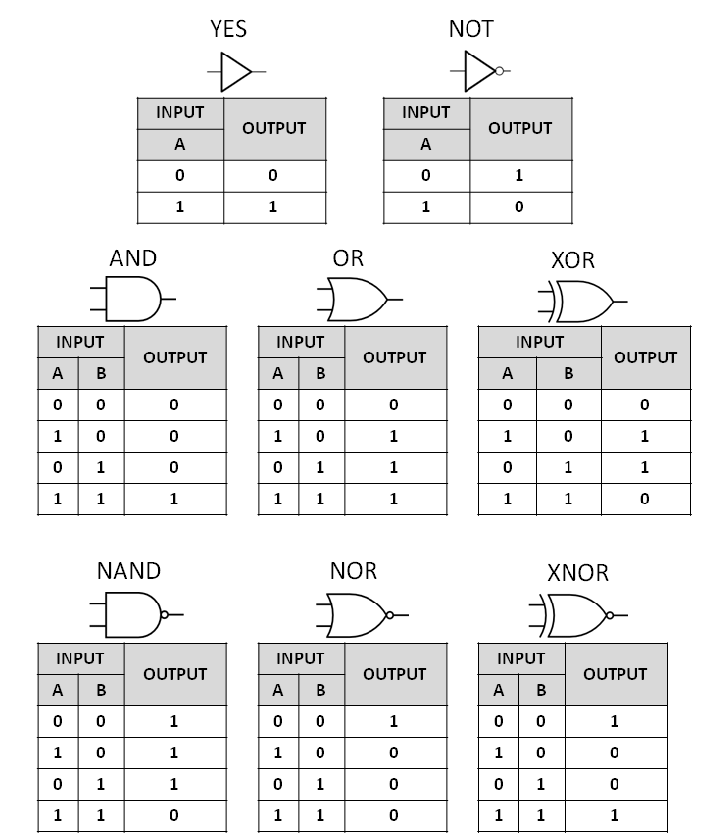
\includegraphics[scale=0.2]{graphics/Summary-of-the-common-Boolean-logic-gates-with-symbols-and-truth-tables.png}
\caption{Bool Gates Trooth Tables}
\label{fig:bool_gate}
\end{wrapfigure}

For the sake of proofing, that the feedforward neural network we have defined is able to be set up, so that for any specific input, any specific output can be obtained. We will view the infrastructure of the weights, bias and the function $\sigma$ together as a circuit. 

\begin{remark}
With circuits you have basic logical gates like AND, OR, and NOT gates and a lot more, that manipulate binary input as shown in figure \ref{fig:bool_gate}. A set of gates is called a Universal Logic Gates Set if with those gates any other logic or Boolean function can be created. After \cite{quine1955way} AND, OR and NOT define such a set. Meaning if we can reproduce these three gates in feedforward neural network form, any boolean logic can be created by these.
%Then again NAND and NOR both can make a AND, OR and NOT gait, so ether of them are so called minimal universal logic gates, meaning they can make any other logic of Boolean function on their own. We will reproduce 




\begin{figure}[H]
    \centering
    \begin{subfigure}[b]{0.3\textwidth}
        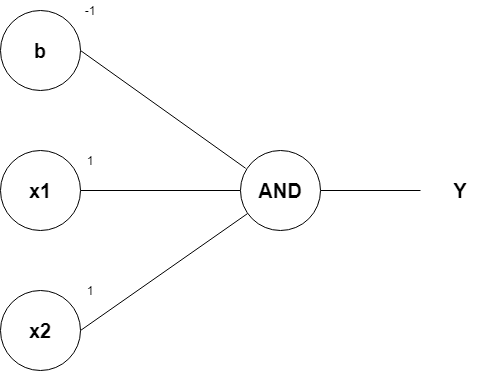
\includegraphics[width=\textwidth]{graphics/AND_gate.png}
        \caption{AND gate}
        \label{fig:AND}
    \end{subfigure}
    \begin{subfigure}[b]{0.3\textwidth}
        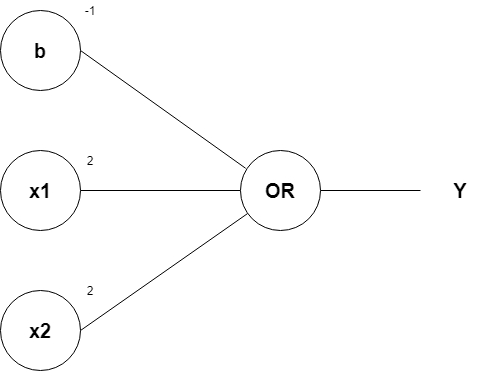
\includegraphics[width=\textwidth]{graphics/OR_gate.png}
        \caption{OR gate}
        \label{fig:OR}
    \end{subfigure}
    \begin{subfigure}[b]{0.3\textwidth}
        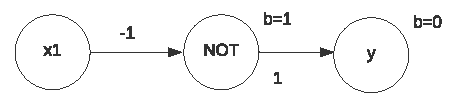
\includegraphics[width=\textwidth]{graphics/NOT_gate.png}
        \caption{NOT gate}
        \label{fig:NOT}
    \end{subfigure}
    \caption{Neural Logical Gates}\label{fig:neural_logic_gates}
\end{figure}

\end{remark}

So now Backpropagation.

\begin{definition}(Backpropagation)
To be defined.
\end{definition}

\begin{remark}
Give an example where backpropagation is used.
Maybe give a code snipped, that does this and add some showcases, since back propagation is not really designed to be done by hand.
\end{remark}

This gives a way to train neural networks on a datapool. \\

The last abstaction level of feedforward neural networks is to define them as function, witch enables to us to compare feedforward neural networds to tropical polynomials in Chapter $4$.

\begin{definition}
Viewed abstractly, an L-layer feedforward neural network is a map $\nu : \mathbb{R}^{d} \to \mathbb{R}^{p}$ given by a composition of functions
$$ \nu = \sigma^{(L)} \circ \rho^{(L)} \circ \sigma^{(L-1)} \circ \rho^{(L-1)} \circ \dots \circ \sigma^{(1)} \circ \rho^{(1)}$$
The preactivation functions $\rho^{(1)}, \dots , \rho^{(L)}$ are affine transformations to be determined and the activation functions $\sigma^{(1)}, \dots , \sigma^{(L)}$ are chosen and fixed in advanced. \\
We denote the width, i.e., the number of nodes, of the $l$th
layer by $n_l, l = 1, \dots , L-1$. We set $n_0 := d$ and $n_L := p$, respectively the dimensions of the input and output of the network. The output from the lth layer will be denoted by
$$\nu = \sigma^{(l)} \circ \rho^{(l)} \circ \sigma^{(l-1)} \circ \rho^{(l-1)} \circ \dots \circ \sigma^{(1)} \circ \rho^{(1)}$$
i.e., it is a map $\nu^{(l)} : \mathbb{R}^{d} \to \mathbb{R}^{n_l}$. For convenience, we assume $\nu^{(0)}(x) := x$. \\
The affine function $\nu^{(l)} : \mathbb{R}^{n_{l-1}} \to \mathbb{R}^{n_{l}}$ is given by a weight matrix $A^{(l)} \in \mathbb{Z}^{n_l \times n_{l-1}} $ and a bias vector $b^{(l)} \in \mathbb{R}^{n_l}$:
$$ \rho^{(l)}(\nu^{(l-1)}) := A^{(l)} \nu{(l-1)} + b{(l)}. $$
The $(i, j)$th coordinate of $A^{(l)}$ will be denoted $a^{l}_{ij}$ and the $i$th coordinate of $b^{(l)}$ by $b^{(l)}_{i}$. Collectively they form the parameters of the $l$th layer
\end{definition}

\begin{comment}
For a vector input $x \in \mathbb{R}^{n_l}, \sigma^{(l)}(x)$ is understood to be in coordinatewise sense; so $\sigma : \mathbb{R}^{n_l} \to \mathbb{R}^{n_l}$. We assume the
final output of a neural network $\nu(x)$ is fed into a score function $s : \mathbb{R}^{p} \to \mathbb{R}^{m}$ that is application specific.
\end{comment}

\begin{comment}
We will make the following mild assumptions
on the architecture of our feedforward neural networks:
\begin{itemize}
\item[(a)]
the weight matrices $Aa^{(1)} , \dots , A^{(L)}$ are integer-valued;
\item[(b)]
the bias vectors $b^{(1)} , \dots , b^{(L)}$ are real-valued;
\item[(c)]
the activation functions $\sigma^{(1)} , \dots , \sigma^{(L)}$ take the form
$$\sigma^{(l)}(x) := \max\{c, t^{(L)}\},$$
where $t^{(l)} \in (\mathbb{R} \cup \{-\infty \})^{n_l}$ is called a threshold vector.
\end{itemize}
Henceforth all neural networks in our subsequent discussions will be assumed to satisfy (a)–(c).
\end{comment}

\newpage

\section{Tropical algebra of neural networks}\label{sec:trop_netw}

\begin{comment}
Consider the output from the first layer in a neural network
$$ \nu(x) = \max \{ Ax+b, t \}; $$
where $A \in \mathbb{Z}^{p \times d}, b \in \mathbb{R}^{p}$, and $t \in (\mathbb{R} \cup \{ Ax + b, t \})$. We will
decompose A as a difference of two nonnegative integervalued matrices, $A = A_{+} - A_{-}$ with $A_{+},A_{-} \in \mathbb{N}^{p \times d}$; e.g., in the standard way with entries
$$ a^{+}_{ij} := \max \{ a_{ij}, 0 \}, \ a^{-}_{ij} := \max \{ -a_ij , 0\} $$
respectively. Since
$$ \max \{ Ax + b, t \} = \max \{ A_{+}x+b, A_{-}x+t \} - A_{-x},$$
we see that every coordinate of one-layer neural network
is a difference of two tropical polynomials.
\end{comment}

For networks with more layers, we apply this decomposition recursively to obtain the following result

\begin{proposition}
Let $A \in \mathbb{Z}^{m \times n}, b \in \mathbb{R}^{m}$ be the parameters of the $(l+1)$th layer, and let $t \in (\mathbb{R} \cup {- \infty})^{m}$ be the threshold vector in the $(l+1)$th layer. If the nodes of the $l$th
layer are given by tropical rational functions,
$$ \nu^{(l)}(x) = F^{(l)}(x) \oslash G^{(l)}(x) = F^{(l)}(x)-G^{(l)}(x),$$
i.e., each coordinate of $f^{(l)}$ and $G^{(l)}$ is a tropical polynomial in $x$, then the outputs of the preactivation and of the $(l+1)$th layer are given by tropical rational functions
\begin{align*}
\rho^{(l+1)} \circ \nu^{(l)}(x) &= H^{(l+1)}(x) - G^{(l+1)}(x), \\
\nu^{(l+1)}(x) = \sigma \circ \rho^{(l+1)} \circ \nu^{(l)}(x) &= F^{(l+1)}(x) - G^{(l+1)}(x),
\end{align*}
respectively, where
\begin{align*}
F^{(l+1)}(x) &= \max \{ H^{(l+1)}(x), G{(l+^)}(x) +t \}, \\
G^{(l+1)}(x) &= A_{x}G^{(l)}(x) + A_{-}F^{(l)}(x), \\
H^{(l+1)}(x) &= A_{+}F^{(l)}(x) + A_{-}G{(l)}(x) +b.
\end{align*}
\end{proposition}

Induction yields the following.

\begin{theorem}
(Tropical characterization of neural networks). \\
A feedforward neural network under assumptions (a)–(c)
is a function $\nu : \mathbb{R}^{d} \to \mathbb{R}^{p}$ whose coordinates are tropical rational functions of the input, i.e.,
$$ \nu(x) = F(x) \oslash G(x) = F(x) - G(x) $$
where $F$ and $G$ are tropical polynomial maps. Thus $\nu$ is a tropical rational map.
\end{theorem}

\begin{comment}
Note that the tropical rational functions above have real coefficients, not integer coefficients. The integer weights $A^(l) \in \mathbb{Z}^{n_l \times n_{l-1}}$ have gone into the powers of tropical monomials in $f$ and $g$, which is why we require our weights to be integer-valued, although as we have explained, this requirement imposes little loss of generality
\end{comment}

By setting $t^{(1)} = \dots = t^{(L-1)} = 0$ and $t^{(l)} = - \infty$, we obtain the following corollary.

\begin{corollary}
Let $\nu : \mathbb{R}^{d} \to \mathbb{R}$ be an ReLU activated feedforward neural network with integer weights and linear output. Then $\nu$ is a tropical rational function.
\end{corollary}

\begin{theorem}
(Equivalence of neural networks and tropical
rational functions).
\begin{itemize}
\item[(i)]
Let $\nu : \mathbb{R}^{d} \to \mathbb{R}$. Then $\nu$ is a tropical rational function if and only if $\nu$ is a feedforward neural network satisfying assumptions (a)–(c).
\item[(ii)]
A tropical rational function $f \oslash g$ can be represented as an $L$-layer neural network, with
$$ L \leq \max \{ \lceil \log_2 r_f \rceil, \lceil \log_2 r_g \rceil \} + 2,$$
where $r_f$ and $r_g$ are the number of monomials in the tropical polynomials $f$ and $g$ respectively.
\end{itemize}
\end{theorem}

\begin{proposition}
Let $\nu : \mathbb{R}^{d} \to \mathbb{R}$. Then $\nu$ is a continuous piecewise linear function with integer coefficients if and only if $\nu$ is a tropical rational function.
\end{proposition}

\begin{comment}
Corollary 5.3, Theorem 5.4, and Proposition 5.5 collectively imply the equivalence of
\begin{itemize}
\item[(i)]
tropical rational functions,
\item[(ii)]
continuous piecewise linear functions with integer coefficients,
\item[(iii)]
neural networks satisfying assumptions (a)-(c).
\end{itemize}
\end{comment}

\begin{proposition}
Every feedforward neural network with ReLU activation is a tropical rational signomial map.
\end{proposition}
\newpage

\bibliographystyle{apacite}
\bibliography{references}

\end{document}